\documentclass{article}
\usepackage[utf8]{inputenc}
\usepackage{amsmath}
\usepackage{amsthm}
\usepackage{amsfonts}
\usepackage{amssymb}
\usepackage{amstext}
\usepackage{gensymb}
\usepackage{graphicx}
\usepackage{enumerate}
\pagenumbering{arabic}
\usepackage{fancyhdr}
\usepackage[margin=0.75in]{geometry}
\usepackage{eucal}
\usepackage{parskip} % removes auto indentation for paragraphs
\usepackage{enumitem} % changes the indexing for enumerate
\setlist[enumerate,1]{label = {(\alph*)}}

\usepackage{listings} % import code into latex

\usepackage{subcaption}

\DeclareMathOperator{\tr}{tr}

\def\N{\mathbb{N}}
\def\Z{\mathbb{Z}}
\def\Q{\mathbb{Q}}
\def\R{\mathbb{R}}
\def\C{\mathbb{C}}
\newcommand{\Mod}[1]{\ (\text{mod}\ #1)}
\newcommand{\Problem}[1]{\textbf{\large Problem #1}}
\newcommand{\li}[0]{\liminf_{n\to\infty}}
\newcommand{\ls}[0]{\limsup_{n\to\infty}}
\newcommand{\dl}[2]{\displaystyle\lim_{#1 \to #2}}
\newcommand{\ds}[2]{\displaystyle\sum_{#1}^{#2}}
\newcommand{\ra}{\Rightarrow}

\linespread{1.5}

\usepackage{float}

\pagestyle{fancy}
\fancyhf{}
\rhead{CSE 6643}
\lhead{Alexander Winkles}
\chead{\Large \textbf{Homework 4}}
\cfoot{Page \thepage}

\begin{document}

\Problem{1}

This MATLAB script computes the pseudoinverse of a matrix $A$ using SVD. 
First the code computes the SVD of $A$.
It then takes the diagonal elements of $S$ and over the next few lines creates the inverse of $S$.
From here it multiplies $VS^{-1}U^T$ to compute the pseudoinverse of $A$. 


\Problem{2}

Consider the following matrices
$$A = \begin{bmatrix} 2 & -1 & 1\\ 1 & 1 & 1\\ 1 & 1 & -2 \end{bmatrix},\ B = \begin{bmatrix} 1 & 2 & -2 \\ 1 & 1 & 1 \\ 2 & 2 & 1 \end{bmatrix}$$
To test if these are convergent for a given method, we much show that $p(G) < 1$, where $G = MN^{-1}$. 
For the Jacobi method, $G = D^{-1}(E + F)$, so we find that
$$G_A = \begin{bmatrix} 0 & 1/2 & -1/2 \\ -1 & 0 & -1 \\ 1/2 & 1/2 & 0 \end{bmatrix},\ G_B = \begin{bmatrix} 0 & -2 & 2 \\ -1 & 0 & -1 \\ -2 & -2 & 0 \end{bmatrix}$$
Thus, we find that $p(G_A) = \frac{\sqrt{5}}{2}$ and $p(G_B) = 0$, so by the theorem from class, the matrix $A$ does not converge and matrix $B$ does. 

For Gauss-Seidel, $G = (D - E)^{-1}F$, so we find that 
$$G_A = \begin{bmatrix} 0 & 1/2 & -1/2 \\ 0 & -1/2 & -1/2 \\ 0 & 0 & -1/2 \end{bmatrix}
G_B = \begin{bmatrix} 0 & -2 & 2 \\ 0 & 2 & -3 \\ 0 & 0 & 2 \end{bmatrix} $$
Thus, we find that $p(G_A) = \frac{1}{2}$ and $p(G_B) = 2$, so by the theorem matrix $A$ will be convergent and matrix $B$ will not be. 

\Problem{3}

Consider the residual of the steepest decent method, so $r_j = b - Ax^{(j)}$.
Thus 
\begin{align*}
r_{j+1} &= b - Ax^{(j+1)} \\
&= b - A(x^{(j)} + \alpha r) \\ 
&= b - A(x^{(j)} + \frac{r^Tr}{r^TAr}r)\\
&= b - Ax^{(j)} - A \frac{r^Tr}{r^TAr}r
\end{align*}
We wish to show that $\left<r_j,r_{j+1}\right> = 0$.
Thus,
\begin{align*}
\left<r_j,r_{j+1}\right> &= (b - Ax^{(j)})^T(b - Ax^{(j)} - A\frac{r_j^Tr_j}{r_j^TAr_j}r_j) \\
&= r_j^Tr_j - (b - Ax^{(j)})^TA\frac{r_j^Tr_j}{r_j^TAr_j}r_j \\
&= r_j^Tr_j - r_j^TA\frac{r_j^Tr_j}{r_j^TAr_j}r_j \\ 
&= r_j^Tr_j - r_j^Tr_j \left(\frac{r_j^TAr_j}{r_j^TAr_j}\right) \\
&= r_j^Tr_j - r_j^Tr_j * 1 \\
&= 0
\end{align*}
\qed

\Problem{4}

Please note that all code being references for problems 4 and 5 may be found at the end of this document.

This problem involved solving $T + \mu I$ matrices of various sizes using the Jacobi, Gauss-Seidel, and SOR methods. 
For each computation, the maximum number of iterations allowed were 50 and the desired error of the solutions were $10^{-10}$. 
For the SOR methods, the relaxation parameter was either $w = 1$ or $w = 1.5$. 
Results for this can be found below:

\begin{figure}[H]
\centering
\caption{Comparing various Iterative Methods for $\mu = 5$ and $\mu = -5$ respectively}
\begin{minipage}[b]{0.4\textwidth}
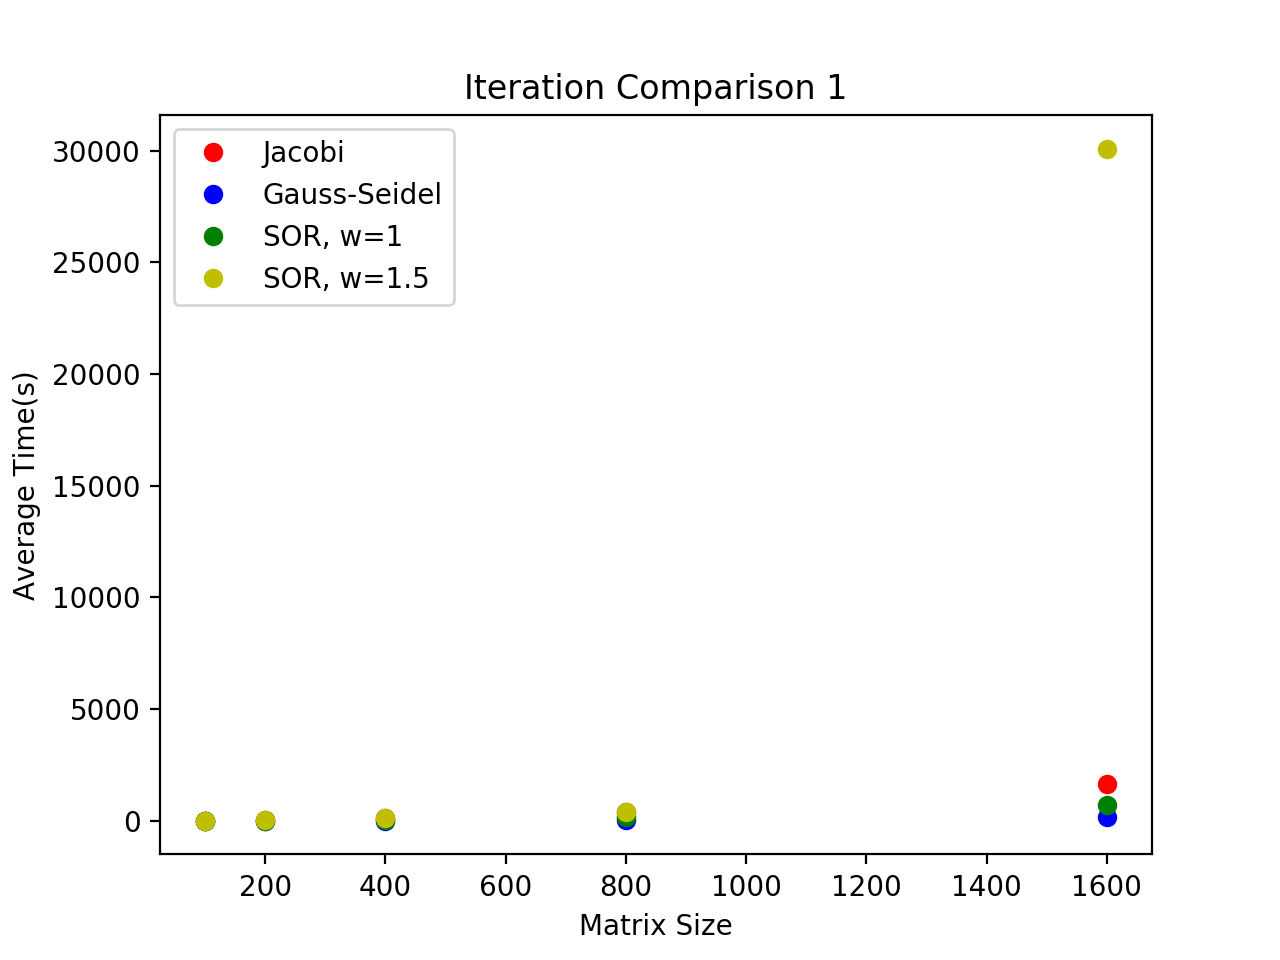
\includegraphics[height=7cm]{p4}	
\end{minipage}
\hspace{0.6in}
\begin{minipage}[b]{0.4\textwidth}
\centering
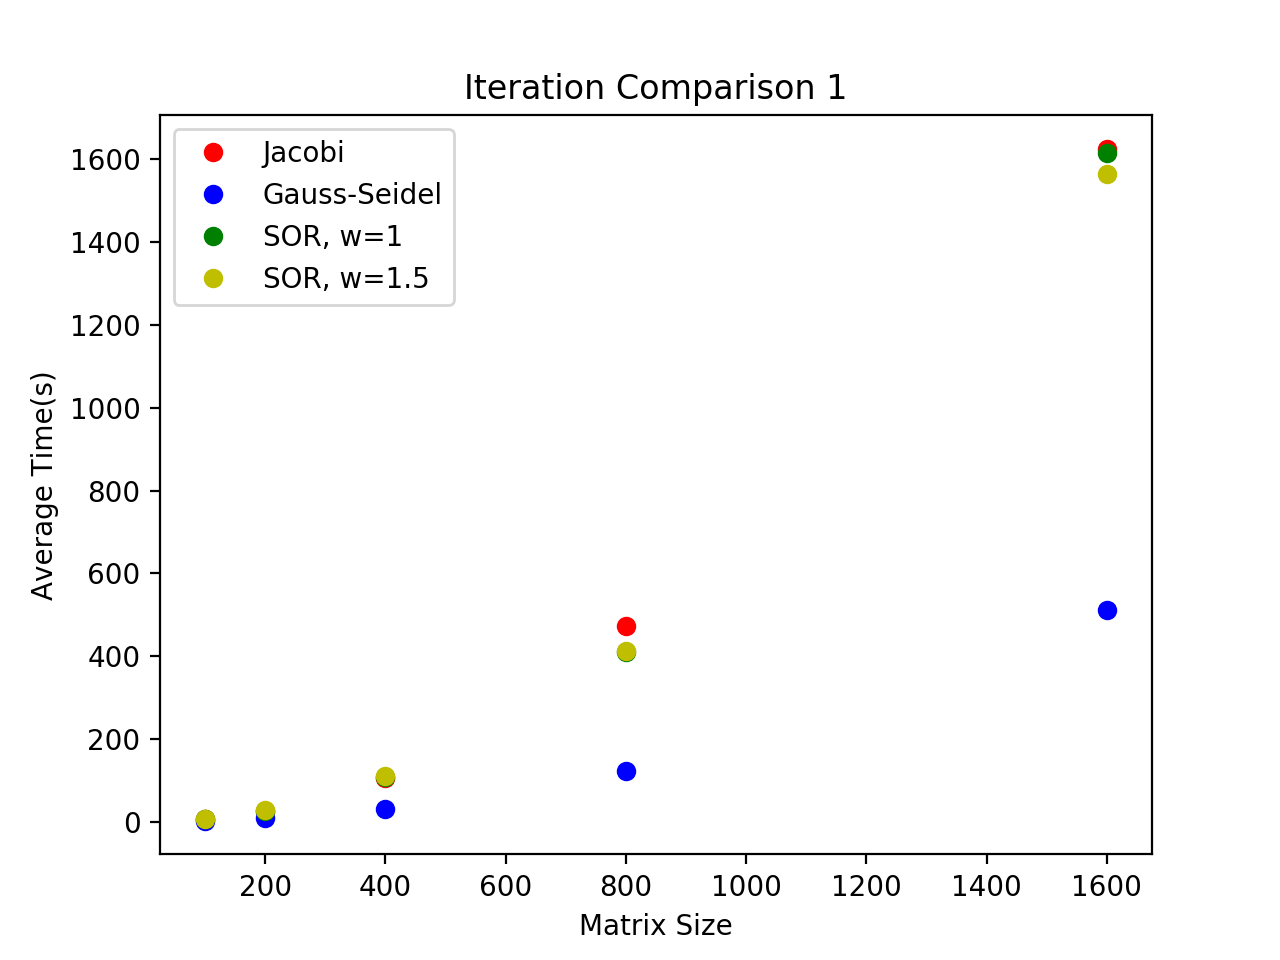
\includegraphics[height=7cm]{p4_2}	
\end{minipage}
\end{figure}

While computing these solutions, the most striking difference was the speed.
For $\mu = 5$, the computations were speedy, especially for the Gauss-Seidel and SOR\textsubscript{w = 1.5} methods, which would terminate before all iterations were necessary. 
Contrasting this, for $\mu = -5$ none of the computations terminated early, which likely means they did not converge to the error desired. 
According to these results, for $\mu = 5$, the fastest method was GS with SOR\textsubscript{w = 1} a close second. 
The slowest method was SOR\textsubscript{w = 1.5}. 
These results make sense, as GS is known to be fast. 
Additionally, since I did not optimize the relaxation parameter and instead chose them at random, the drastic speed difference between the two SOR instances makes sense. 
Had an optimized relaxation parameter been utilized, SOR would no doubt have been the fastest.
For $\mu = -5$, the solutions took far longer to compute. 
I imagine this it due to many of the vectors not converging, which may be a result of the $\mu$ value changing the spectral radius of the matrices.
Additionally, this change in matrix led to the relaxation parameter 1.5 to be more optimized for the problem, while the relaxation parameter 1.0 was less optimized.
Regardless, the GS method still reigned supreme in speed compared to other results. 
 

\Problem{5}

For this problem, I was tasked to solve the following differential equation using the Steepest Descent and Conjugate Gradient methods:
$$\begin{cases} -u'' + \lambda u = 3x - \frac{1}{2} \quad x\in [0,1] \\ u(0) = 0,\ u(1) = -2 \end{cases}$$
This task proved to be more difficult than expected. 
For whatever reason, the solutions vectors for this problem would not converge, despite great refinement of the mesh. 
In this, 2000 iterations were done with an error cutoff of $10^{-5}$ (which was never obtained in the 2000 iterations). 
Because of this, the algorithm solutions do not match the ``true'' solution exactly, as seen in the figures below. 
I found my code to be inconsistent; sometimes it would accurately match the true solution and sometimes it would be completely off. 
I believe this greatly depends on the size of the matrix and the number of iterations, as smaller matrices actually led to more accurate results. 

\begin{figure}[H]
\centering
\caption{Time Comparison between methods}
\begin{minipage}[b]{0.4\textwidth}
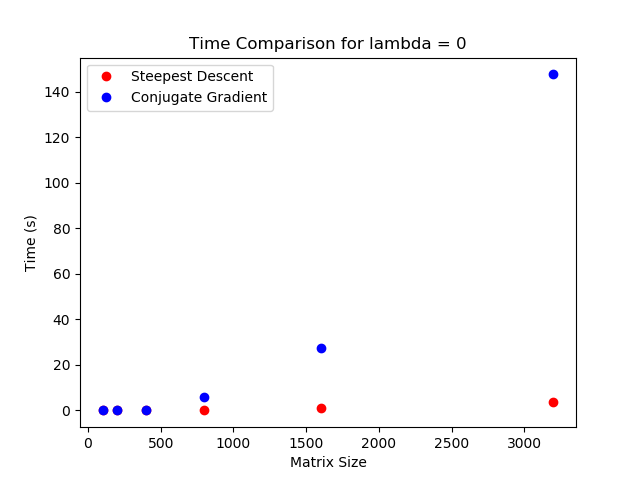
\includegraphics[height=7cm]{time0}	
\end{minipage}
\hspace{0.6in}
\begin{minipage}[b]{0.4\textwidth}
\centering
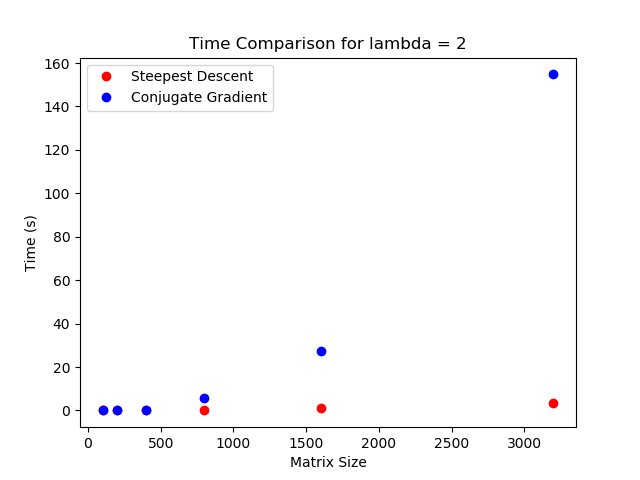
\includegraphics[height=7cm]{time2}	
\end{minipage}
\end{figure}

\begin{figure}[H]
\centering
\caption{Comparing Steepest Descent to Exact Solution}
\begin{minipage}[b]{0.4\textwidth}
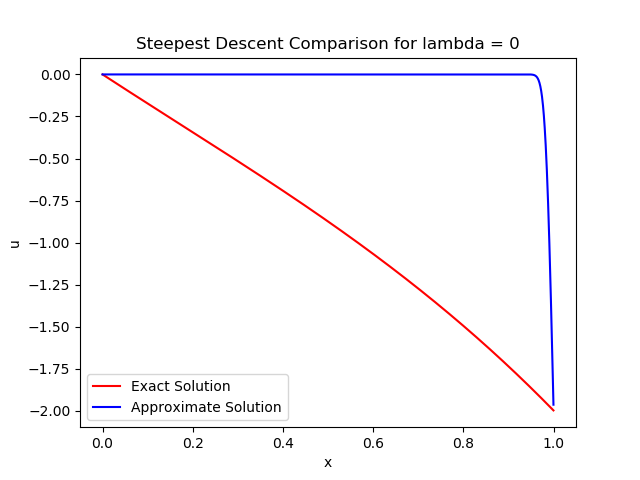
\includegraphics[height=7cm]{sd0}	
\end{minipage}
\hspace{0.6in}
\begin{minipage}[b]{0.4\textwidth}
\centering
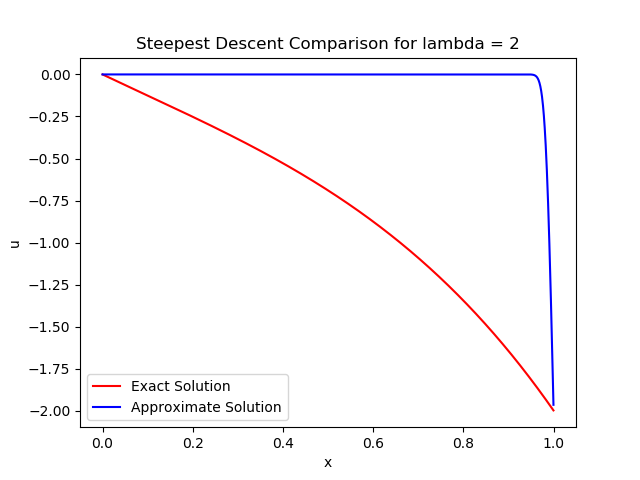
\includegraphics[height=7cm]{sd2}	
\end{minipage}
\end{figure}

\begin{figure}[H]
\centering
\caption{Comparing Conjugate Gradient to Exact Solution}
\begin{minipage}[b]{0.4\textwidth}
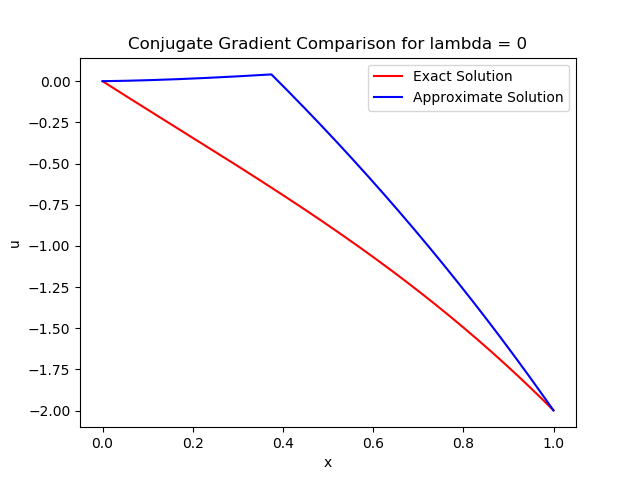
\includegraphics[height=7cm]{cg0}	
\end{minipage}
\hspace{0.6in}
\begin{minipage}[b]{0.4\textwidth}
\centering
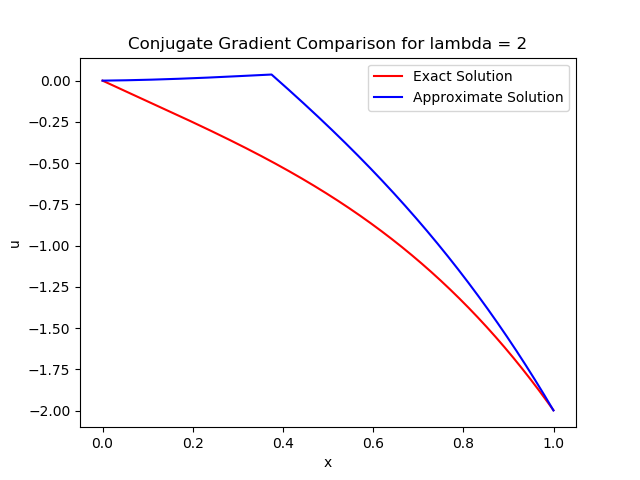
\includegraphics[height=7cm]{cg2}	
\end{minipage}
\end{figure}

\begin{figure}[H]
\centering
\caption{Conjugate Gradient Method for 200 x 200 matrix with 2000 iterations}
\begin{minipage}[b]{0.4\textwidth}
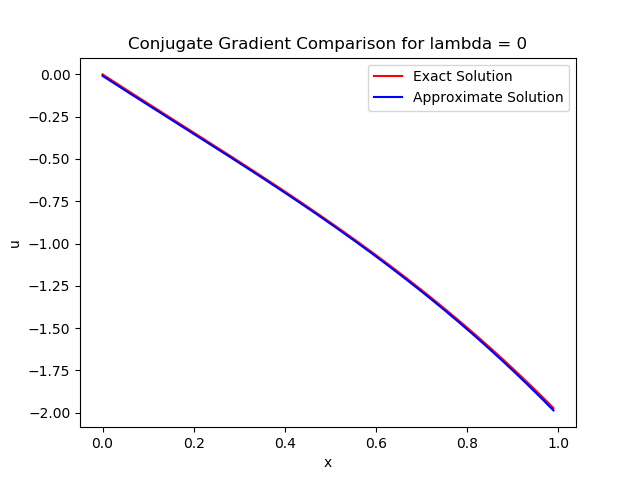
\includegraphics[height=7cm]{goodcg0}	
\end{minipage}
\hspace{0.6in}
\begin{minipage}[b]{0.4\textwidth}
\centering
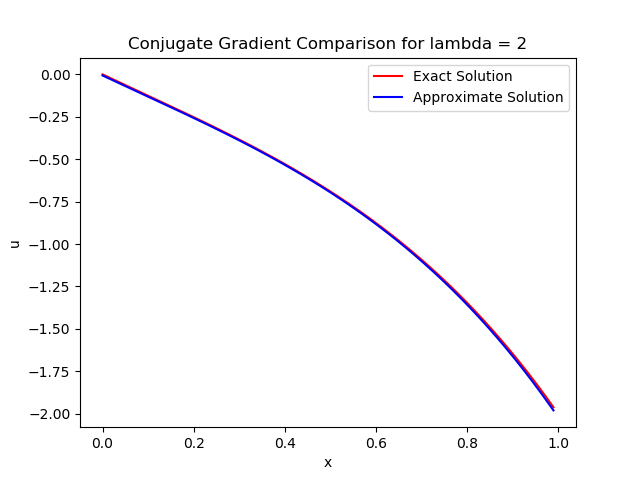
\includegraphics[height=7cm]{goodcg2}	
\end{minipage}
\end{figure}

As seen above, for certain parameters the conjugate gradient method was able to approximate the exact solution well, but for other parameters not so much. 
On the other hand, steepest descent never converged and thus did not achieve results near the exact solution. 
However, steepest descent did run far faster than conjugate gradient as seen in Figure 1. 

\Problem{Code}

\lstinputlisting[language=Python]{"iteration.py"}
\lstinputlisting[language=Python]{"matrixgen.py"}



\end{document}
